\subsection{Sample Memory Distribution} \label{subsec:Sample_Memory_Distribution} 
The ADC converters output are 16 bit sample values and the IS61 external SRAM being used in the project can store 8 bit values, so the 16 bit sample values must be mapped into two 8 bit values in order to be stored in the external memory. The function of the Sample Memory Distribution(SMD) submodule is to split the 16 bit word into two bytes and clock it into, and out of, memory through the read/write module described in section \refq{subsec:Sample_Memory}.

For both read and write operations the SMD module will split the incoming 16 bit sample and address into a \textit{high byte} and \textit{low byte} value and map the values to a 19 bit address as shown on figure \refq{fig:7_2_6_MemDist}.

\begin{figure}[H]
    \centering
    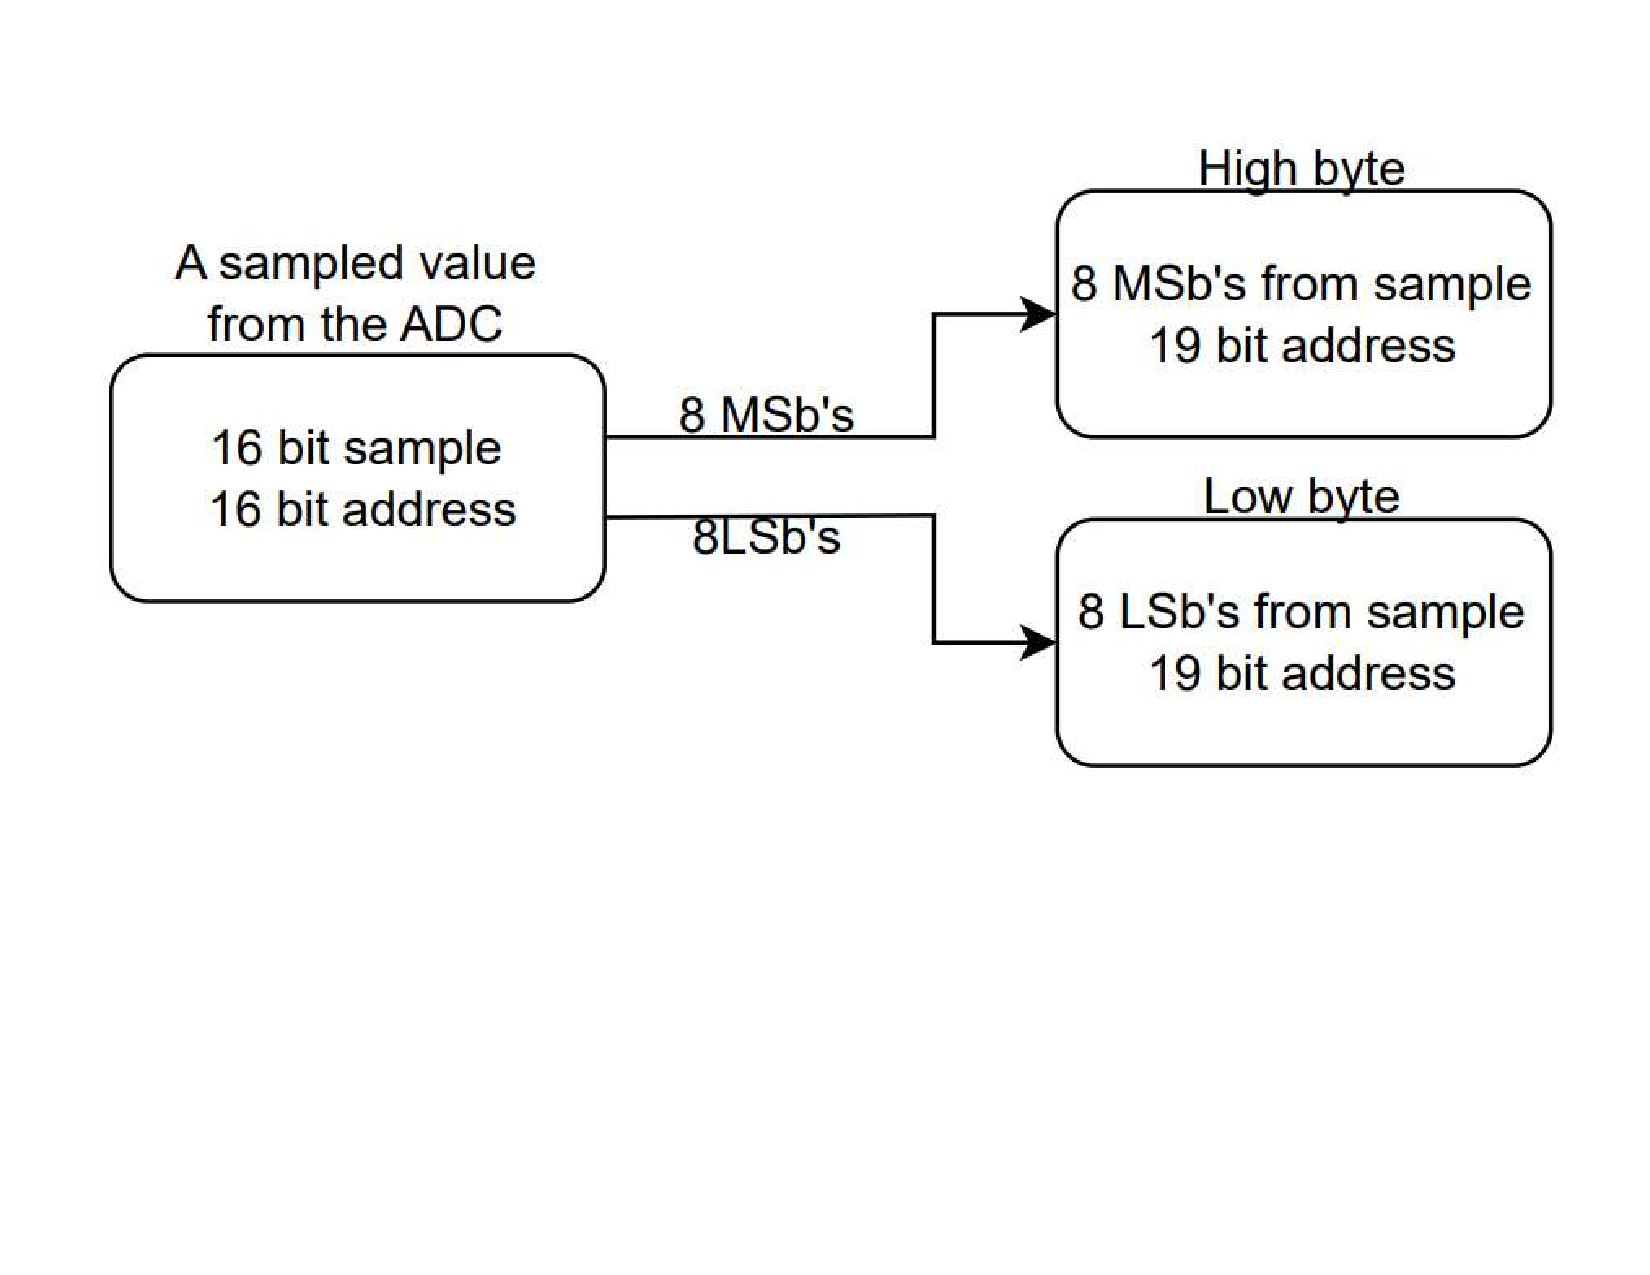
\includegraphics[clip, trim=0 220 0 0, width=0.55\textwidth]{Sections/7_SystemDesign/Figures/7_2_6_1_MemoryDist.pdf}
    \caption{The module will split an incoming 16 bit word into two bytes and map the address to the 19 bits that the IS61 memory requires.}
    \label{fig:7_2_6_MemDist}
\end{figure}

The IS61 has a 19 bit address bus as shown in section \refq{subsec:Sample_Memory} and the memory has been effectively split in half where the upper part will store the high byte values and the lower part will stort the low byte values. This has been done by turning the 19th bit into a sign bit that indicates whether, or not, a value is the 8 MSbs or LSBs from the sample as shown in code listing \refq{lst:7_2_6_SMD}.

\lstinputlisting[language=C ,style = c,firstnumber=1, linerange=94-107, caption={VHDL code for the write sequence state machine}, label={lst:7_2_6_SMD}]{Sections/7_SystemDesign/Code/ExternalMemoryControl.vhd}

The code listing starts by splitting the incoming sample value up into a it's 8 LSbs and 8 MSbs.
The code listing will start by splitting the incoming 16 bit sample value into a high byte that contains the 8 MSbs from the sample and a low byte that contains the 8 LSBs from the sample. It will, when triggered by a CLK, concatenate the incoming address from the IV Saver module with "000" to form a 19 bit address for the low byte and "100" for the high byte address.

Note how the signal names in the process are \textit{long}, this is a common theme in all the VHDL code listings in this project. It was found to be significantly easier to integrate the various VHDL modules in a single top layer when all signals, especially in/out signals from a VHDL block, with other VHDL blocks when all the signals are explicitly saying where they are supposed to connect to other blocks.

To write, or read, to memory the Sample Memory Distribution module will have to clock the data into the read/write interface shown in section \refq{subsec:Sample_Memory} twice. One for the high hyte and one for the low byte. This is done with, yet another, clocked state machine that can seen in appendix \refq{App:MemoryDistributionCode}.

